\section{Evaluation}
\label{sec:evaluation}

\subsection{Experiment 1: Representative operating points}

Figure~\ref{fig:rep} is the paper's trajectory-level visualization figure. The top row shows representative seed traces and the bottom row shows all 20 seed-level test outcomes. This figure is useful because it makes the failure modes legible: Raw is often too noisy, EV is cleaner but can over-smooth or miss amplitude, and Split lands between them.

All three representative panels now use exactly the same operating point ($Q=4$, $N_{\mathrm{shots}}=18$, $\sigma=0$, $\lambda=10$, $\rhoEV=2.65125$), so the visual comparison is no longer entangled with task-specific choices. At this common operating point, the 20-seed test $\NRMSE$ values are:
\begin{itemize}[leftmargin=*]
    \item \textbf{Mackey--Glass:} EV $0.446\pm0.103$, Raw $0.563\pm0.076$, Split $0.414\pm0.072$;
    \item \textbf{Lorenz:} EV $0.925\pm0.168$, Raw $0.990\pm0.126$, Split $0.845\pm0.142$;
    \item \textbf{NARMA10:} EV $0.947\pm0.098$, Raw $0.911\pm0.027$, Split $0.863\pm0.035$.
\end{itemize}
The paired statistics are cleaner than mean$\pm$standard deviation alone. Split improves on EV by $\Delta=0.032\pm0.018$ (95\% CI half-width), with win-rate $0.75$ and Wilcoxon $p=2.7\times10^{-3}$ on Mackey--Glass, by $\Delta=0.080\pm0.055$ with win-rate $0.90$ and $p=4.2\times10^{-3}$ on Lorenz, and by $\Delta=0.084\pm0.034$ with win-rate $0.85$ and $p=3.6\times10^{-5}$ on NARMA10. Raw is already below EV on NARMA10 at this shared operating point, so the claim here is intentionally narrower than universal dominance: under matched budget, Split is the best overall protocol across the three tasks, while Figure~\ref{fig:gap} remains the actual regime test. This common operating point is also not an artifact of one favorable ridge choice: Appendix Experiment~8 (Figure~\ref{fig:applambdafig}) shows that the Split-versus-EV ordering is unchanged across the full shared $\lambda$ grid.

\begin{figure*}[!t]
    \centering
    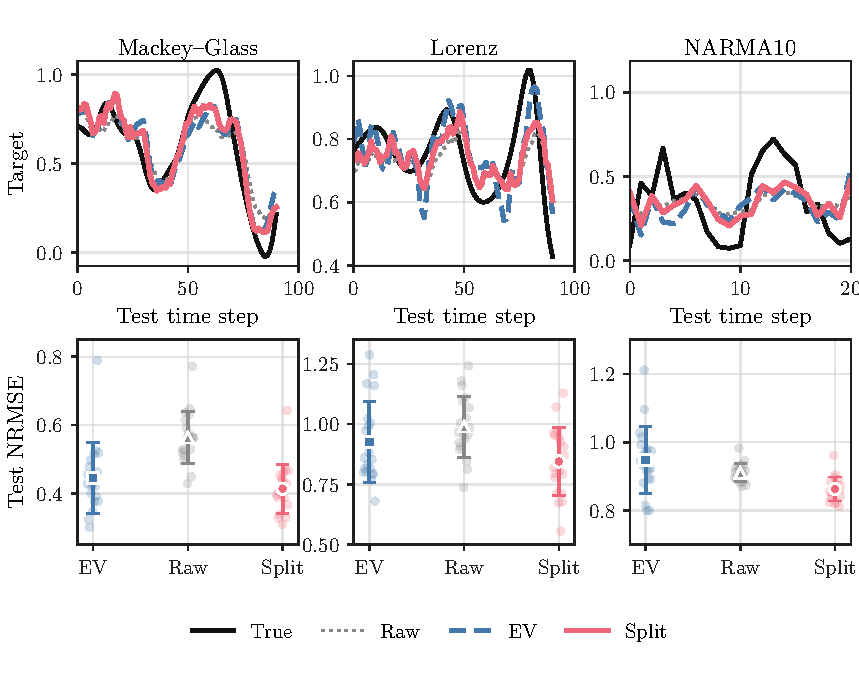
\includegraphics[width=0.985\textwidth]{experiment_1.pdf}
    \caption{Common operating point comparison. Top row: one representative seed trajectory per benchmark, chosen as the seed whose Split test $\NRMSE$ is closest to the 20-seed median. Bottom row: all 20 seed outcomes with the sample mean and standard deviation. All three tasks use the same synthetic operating point ($Q=4$, $N_{\mathrm{shots}}=18$, $\sigma=0$, $\lambda=10$), which makes the comparison visually uniform and easy to audit.}
    \label{fig:rep}
\end{figure*}

\subsection{Experiment 2: Empirical regime test versus \texorpdfstring{$\rhoEV$}{rho-EV}}

Figure~\ref{fig:gap} is the paper's main regime plot. The theory in Section~\ref{sec:methodology} says that grouping gives an exact right-shift in aspect ratio and that this shift should matter most when EV is still row-limited. Figure~\ref{fig:gap} tests exactly that idea on the common synthetic sweep over $\rhoEV$.

Three observations matter. First, the displayed mean gap is positive for all shown Lorenz and NARMA10 points and for the shown Mackey--Glass points. Second, the advantage is generally larger at smaller to intermediate $\rhoEV$ than in the better-conditioned range. Third, as $\rhoEV$ increases, the gap shrinks toward zero rather than growing. The peak paired deltas quantify this directly: on Mackey--Glass the largest effect occurs at $N_{\mathrm{shots}}=50$ ($\rhoEV=0.7875$) with $\Delta=0.335\pm0.102$, win-rate $0.95$, and Wilcoxon $p=3.8\times10^{-6}$; on Lorenz at $N_{\mathrm{shots}}=25$ ($\rhoEV=1.8375$) with $\Delta=0.451\pm0.221$, win-rate $0.95$, and $p=3.6\times10^{-5}$; and on NARMA10 at $N_{\mathrm{shots}}=40$ ($\rhoEV=1.05$) with $\Delta=0.648\pm0.228$, win-rate $1.00$, and $p=1.9\times10^{-6}$. That is the regime picture the paper needs: grouping helps most when EV is still row-limited; once EV is comfortably conditioned, the extra grouped views matter less.

\begin{figure}[!t]
    \centering
    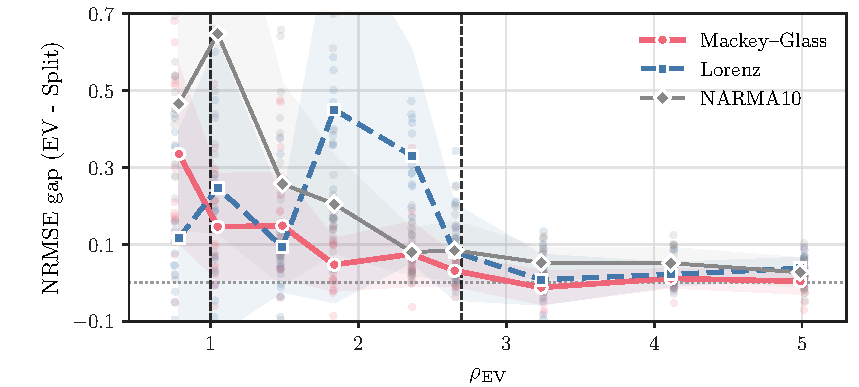
\includegraphics[width=0.98\columnwidth]{experiment_2.pdf}
    \caption{Empirical split gain along the common synthetic sweep. Faint background points show individual seeds; solid lines with translucent bands show the 20-seed mean and standard deviation. The main lesson is not a universal numeric threshold but a clear regime trend: Split helps most when EV is still relatively row-limited, and the gain shrinks as $\rhoEV$ grows.}
    \label{fig:gap}
\end{figure}

\subsection{Experiment 4: Stronger protocol and estimator controls}

Figure~\ref{fig:base} compares Split not only to EV and Raw but also to EV-dup, EV-NA, and Split-NA. This is the main reviewer-facing control figure because it asks whether the effect can be explained away by matching the grouped row count or by adding a simple variance-aware penalty.

Under the same common operating point, the answer is favorable but should be stated precisely. Split is the lowest-mean \emph{plain} protocol on Mackey--Glass, Lorenz, and NARMA10. Against EV-dup, the paired deltas remain positive on all three datasets: $\Delta=0.032$ on Mackey--Glass, $\Delta=0.071$ on Lorenz, and $\Delta=0.103$ on NARMA10; Lorenz is the weakest of the three controls (win-rate $0.65$, Wilcoxon $p=5.8\times10^{-2}$, paired $t$-test $p=4.6\times10^{-2}$), but the direction remains the same. EV-NA likewise does not close the gap. The only near-tie is Split-NA, where the differences are numerically tiny (order $10^{-5}$ to $10^{-3}$). The claim that survives these controls is therefore the one we actually need: shot organization is a real design variable, and grouped views outperform simple row-count matching while remaining competitive with a diagonal noise-aware proxy under the same shared synthetic setup.

\begin{figure*}[!t]
    \centering
    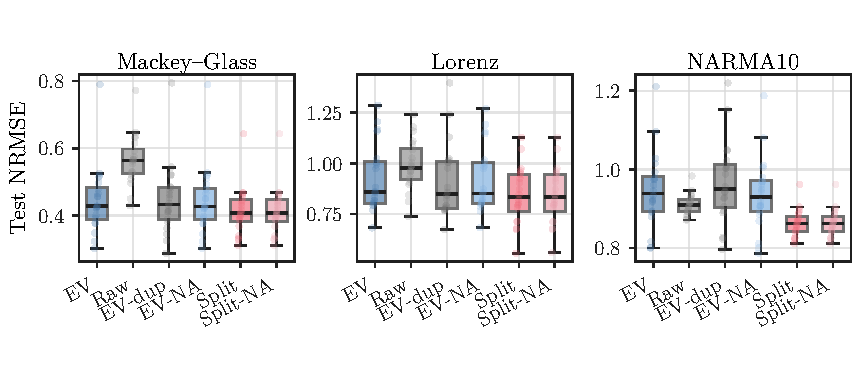
\includegraphics[width=0.985\textwidth]{experiment_4.pdf}
    \caption{Baseline controls at the common operating point. EV-dup tests whether the gain is explained solely by row-count matching; EV-NA and Split-NA test a simple diagonal variance-aware penalty. Split remains the strongest plain protocol across all three benchmarks under the same shared synthetic setting and is effectively tied with the diagonal Split-NA proxy.}
    \label{fig:base}
\end{figure*}

\subsection{Hardware validation on IBM Quantum}

The synthetic narrative would be incomplete without a device-level check because the whole point of the protocol is to make fixed shot budgets count on real hardware. We therefore import the hardware experiment from the companion study on \texttt{ibm\_marrakesh}. This is a deliberately modest hardware claim: one task, one backend, one shot-limited operating point, no error mitigation. That is enough for our purpose because the paper's main claim is about \emph{protocol behavior under real shot noise}, not about broad hardware supremacy.

The result is strong. On Mackey--Glass with the same hardware shot records for all methods, EV gives $\NRMSE=1.023\pm0.235$, Raw gives $0.932\pm0.021$, and Split gives $0.670\pm0.080$. That corresponds to an absolute gap of $0.353$ versus EV and preserves the same ranking seen in the synthetic study.

\begin{table}[!t]
    \caption{Hardware summary on \texttt{ibm\_marrakesh} (Mackey--Glass, $\Stotal=20$k, $N_{\mathrm{shots}}=40$, 8 seeds).}
    \label{tab:hardware}
    \centering
    \begin{tabular}{lcc}
        \toprule
        Protocol & Test $\NRMSE$ & Best $k$ / grouping \\
        \midrule
        EV & $1.023 \pm 0.235$ & $k=40$ \\
        Raw & $0.932 \pm 0.021$ & $k=1$ \\
        Split & $0.670 \pm 0.080$ & $k=10$ \\
        \bottomrule
    \end{tabular}
\end{table}

\subsection{Scaling the reservoir}

The appendix enlarges the reservoir while keeping the protocol fixed. Figure~\ref{fig:appmoreq} now sweeps all three tasks through $Q=12$ with $20$ seeds per point and yields a cleaner result than before: the paired EV-minus-Split delta is positive in all $15/15$ reported size cells and Wilcoxon-significant in $14/15$. On Mackey--Glass the mean gap rises from $0.042$ at $Q=4$ to a maximum of $0.299$ at $Q=8$ and stays positive through $Q=12$ at $0.194$; on NARMA10 it rises from $0.113$ at $Q=4$ to $0.600$ at $Q=12$. Lorenz is no longer the weak case: the mean delta is already $0.254$ at $Q=4$, grows to $0.732$ at $Q=10$, and remains $0.404$ at $Q=12$, with all five Lorenz size cells paired-significant.

This appendix matters for two reasons. First, it answers the natural objection that a four-qubit reservoir is too small for the conditioning story to be meaningful. Second, it shows that the protocol effect is not washed out as the readout dimension increases. In that sense the larger-reservoir sweep is not decorative; it materially strengthens the practical relevance of the paper.

\subsection{What the theory adds and what it does not}

Theoretical restraint is a feature here. The exact grouped-view lift, the attenuation factor, and the warm-start $k_\star$ are the parts of the theory that are actually useful. They motivate the regime picture and yield a practical decision rule. The paper does \emph{not} need a universal theorem for test error or a universal numeric crossover. The evidence for lower test error is empirical, and it is strongest exactly where the theory predicts the conditioning gain should matter most.
